% Options for packages loaded elsewhere
\PassOptionsToPackage{unicode}{hyperref}
\PassOptionsToPackage{hyphens}{url}
%
\documentclass[
  12pt,
]{article}
\usepackage{lmodern}
\usepackage{amssymb,amsmath}
\usepackage{ifxetex,ifluatex}
\ifnum 0\ifxetex 1\fi\ifluatex 1\fi=0 % if pdftex
  \usepackage[T1]{fontenc}
  \usepackage[utf8]{inputenc}
  \usepackage{textcomp} % provide euro and other symbols
\else % if luatex or xetex
  \usepackage{unicode-math}
  \defaultfontfeatures{Scale=MatchLowercase}
  \defaultfontfeatures[\rmfamily]{Ligatures=TeX,Scale=1}
\fi
% Use upquote if available, for straight quotes in verbatim environments
\IfFileExists{upquote.sty}{\usepackage{upquote}}{}
\IfFileExists{microtype.sty}{% use microtype if available
  \usepackage[]{microtype}
  \UseMicrotypeSet[protrusion]{basicmath} % disable protrusion for tt fonts
}{}
\makeatletter
\@ifundefined{KOMAClassName}{% if non-KOMA class
  \IfFileExists{parskip.sty}{%
    \usepackage{parskip}
  }{% else
    \setlength{\parindent}{0pt}
    \setlength{\parskip}{6pt plus 2pt minus 1pt}}
}{% if KOMA class
  \KOMAoptions{parskip=half}}
\makeatother
\usepackage{xcolor}
\IfFileExists{xurl.sty}{\usepackage{xurl}}{} % add URL line breaks if available
\IfFileExists{bookmark.sty}{\usepackage{bookmark}}{\usepackage{hyperref}}
\hypersetup{
  pdftitle={Welcome Home --- Now Vote!},
  pdfauthor={Kevin Morris},
  hidelinks,
  pdfcreator={LaTeX via pandoc}}
\urlstyle{same} % disable monospaced font for URLs
\usepackage[margin=1in]{geometry}
\usepackage{longtable,booktabs}
% Correct order of tables after \paragraph or \subparagraph
\usepackage{etoolbox}
\makeatletter
\patchcmd\longtable{\par}{\if@noskipsec\mbox{}\fi\par}{}{}
\makeatother
% Allow footnotes in longtable head/foot
\IfFileExists{footnotehyper.sty}{\usepackage{footnotehyper}}{\usepackage{footnote}}
\makesavenoteenv{longtable}
\usepackage{graphicx}
\makeatletter
\def\maxwidth{\ifdim\Gin@nat@width>\linewidth\linewidth\else\Gin@nat@width\fi}
\def\maxheight{\ifdim\Gin@nat@height>\textheight\textheight\else\Gin@nat@height\fi}
\makeatother
% Scale images if necessary, so that they will not overflow the page
% margins by default, and it is still possible to overwrite the defaults
% using explicit options in \includegraphics[width, height, ...]{}
\setkeys{Gin}{width=\maxwidth,height=\maxheight,keepaspectratio}
% Set default figure placement to htbp
\makeatletter
\def\fps@figure{htbp}
\makeatother
\setlength{\emergencystretch}{3em} % prevent overfull lines
\providecommand{\tightlist}{%
  \setlength{\itemsep}{0pt}\setlength{\parskip}{0pt}}
\setcounter{secnumdepth}{5}
\usepackage{rotating}
\newcommand{\beginsupplement}{\setcounter{table}{0}  \renewcommand{\thetable}{A\arabic{table}} \setcounter{figure}{0} \renewcommand{\thefigure}{A\arabic{figure}}}
\usepackage{booktabs}
\usepackage{longtable}
\usepackage{array}
\usepackage{multirow}
\usepackage{wrapfig}
\usepackage{float}
\usepackage{colortbl}
\usepackage{pdflscape}
\usepackage{tabu}
\usepackage{threeparttable}
\usepackage{threeparttablex}
\usepackage[normalem]{ulem}
\usepackage{makecell}
\usepackage{xcolor}
\newlength{\cslhangindent}
\setlength{\cslhangindent}{1.5em}
\newenvironment{cslreferences}%
  {\setlength{\parindent}{0pt}%
  \everypar{\setlength{\hangindent}{\cslhangindent}}\ignorespaces}%
  {\par}

\title{Welcome Home --- Now Vote!\thanks{Prepared for the 2020 Annual Meeting of the Midwest Political Science Association. The author thanks Jacob Faber, Jeff Manza, Myrna Pérez, Ariel White, and Peter Miller for their comments on this project. All errors are my responsibility.}}
\usepackage{etoolbox}
\makeatletter
\providecommand{\subtitle}[1]{% add subtitle to \maketitle
  \apptocmd{\@title}{\par {\large #1 \par}}{}{}
}
\makeatother
\subtitle{Voting Rights Restoration and Post-Supervision Participation}
\author{Kevin Morris\footnote{Researcher, Brennan Center for Justice at NYU School of Law, 120 Broadway Ste 1750, New York, NY 10271 (\href{mailto:kevin.morris@nyu.edu}{\nolinkurl{kevin.morris@nyu.edu}})}}
\date{January 23, 2020}

\begin{document}
\maketitle
\begin{abstract}
This paper presents causal estimates of the effect of voting rights restoration prior to discharge from parole on post-supervision participation. In 2018, New York State began restoring voting rights to parolees, after previously restoring voting rights only at the completion of parole. By leveraging randomness in parole discharge date, I interrogate whether restoring voting rights to parolees increases their post-supervision propensity to cast a ballot. I demonstrate that individuals whose rights were restored while still on parole were more likely to participate than those whose rights were automatically restored upon completion of parole. This group-level effect, however, masks race-specific effects. Although rights restoration prior to parole discharge effectively doubled turnout among white former parolees, it had no measurable effect on the turnout of non-white former parolees. This raises serious questions about how rights restoration programs are implemented, and how incarceration might differently structure black Americans' view of the democratic process.
\end{abstract}

\pagenumbering{gobble}
\pagebreak

\pagenumbering{arabic}

\hypertarget{introduction}{%
\section*{Introduction}\label{introduction}}
\addcontentsline{toc}{section}{Introduction}

In all but two states (Maine and Vermont), felony disenfranchisement laws mean that American citizens convicted of felony offenses lose the right to vote for at least some period of time. In some states, such as Oregon and Massachusetts, individuals lose that right only for the period in which they are actively incarcerated. In other states, notably Kentucky and Iowa, felony convictions result in lifelong disenfranchisement unless a returned citizen receives an individual pardon from the state's governor (Brennan Center for Justice \protect\hyperlink{ref-bcj_laws}{2018}). This variation in laws arises from language in the Fourteenth Amendment which allows states to revoke individuals' voting rights ``for participation in rebellion, or other crime.'' The definition of ``other crime,'' left so vague in the Constitution, is now generally used by states to disenfranchise citizens for any felony offense. The Supreme Court, in cases such as \emph{Richardson v. Ramirez} (1974), has upheld states' right to do just that. Collectively, these laws disenfranchise as many as 4.7 million American citizens. Of these, the majority are no longer incarcerated, but are living and working in their communities (Uggen, Larson, and Shannon \protect\hyperlink{ref-sentencing_2016}{2016}).\footnote{The figures reported in Uggen, Larson, and Shannon (\protect\hyperlink{ref-sentencing_2016}{2016}) have been adjusted to reflect the impact of Amendment 4 in Florida.}

There is some evidence that incarceration continues to structure political participation even after an individual is no longer legally disenfranchised. As previous literature has established, interactions with the criminal justice system leaves residents less likely to vote in the future (White \protect\hyperlink{ref-White2019}{2019}; but see Gerber et al. \protect\hyperlink{ref-Gerber2017}{2017}). As Burch (\protect\hyperlink{ref-Burch2011}{2011}) and others have shown, moreover, turnout rates among the formerly incarcerated are extremely low. Formal disenfranchisement policy, the literature has made clear, is just one piece of an interlocking system that serves to disenfranchise minority and marginalized voters. The incarcerated population is drawn from a pool of individuals unlikely to vote even prior to their incarceration. To address only the formal laws contributing to disenfranchisement without also interrogating efforts to boost post-supervision participation risks leaving much of the system of effective disenfranchisement undisturbed. New York State offers us the opportunity to test how the timing of the re-instation of voting rights structures post-supervision participation.

Prior to 2018, New Yorkers convicted of felony offenses and sentenced to prison were disenfranchised until they had completed all terms of their sentence --- their period of incarceration as well as any parole term. For New Yorkers on life parole or sentenced to life in prison, this law resulted in effective lifetime disenfranchisement. New Yorkers sentenced to felony probation, on the other hand, did not lose their voting rights.

On April 18\textsuperscript{th}, 2018, Governor Andrew Cuomo signed Executive Order 181 which effectively ended the disenfranchisement of New Yorkers on parole. Such a move was of course good for individuals who were still on parole on election day, and would have been disenfranchised otherwise. The change in policy is also beneficial for felony probationers: despite the fact that probationers do not formally lose their voting rights, there is evidence that confusion around the law contributes to \emph{de facto} disenfranchisement among probationers (Drucker and Barreras \protect\hyperlink{ref-Drucker2005}{2005}). The executive order is a promising step: by changing the policy to allow all New York citizens living in their communities to cast a ballot, the move has the potential to both re-enfranchise the nearly 30,000 New Yorkers on parole living in the community and to clarify the rules about who is eligible to vote.

There is reason to believe that the executive order may also have increased the political participation of formerly disenfranchised individuals. Prior to the policy change, formerly incarcerated individuals had their voting rights restored automatically upon the completion of their parole term. New York's correction code provides no more guidance other than that ``upon a person's discharge from community supervision, the department shall notify such person of his or her right to vote and provide such person with a form of application for voter registration'' (Section 75 of the New York State Correction Law). Shortly after the implementation of the executive order, Acting Deputy Commissioner for Community Supervision Ana Enright sent a memorandum to New York State parole officers detailing the Department of Corrections' new approach.\footnote{Link: \url{https://nyassembly.gov/member_files/139/webdocs/82103.pdf}} The memorandum directs all parole officers to present parolees with voter registration forms and to explain their purpose. Parole officers were also instructed to offer any assistance needed, including help filling out the registration form. In addition to these directives, the memorandum communicates that voter registration is to receive ``high priority attention,'' and it separately calls the program ``a \textbf{priority} initiative'' {[}emphasis in the original{]}. Thus, the executive order demands not only that re-enfranchised individuals receive in-person notification of their voting rights, but also that parole officers prioritize their registration.

In the analysis below, I examine the effect of Executive Order 181 on individuals who finished parole before October 10\textsuperscript{th}, 2018 (the registration deadline for 2018). These individuals, because they were discharged from parole before the registration deadline, would have been eligible to vote even in the absense of the executive order. This is only a subset of the individuals who were impacted by Executive Order 181 --- many of the individuals who had their voting rights restored were still on parole on election day, and therefore were eligible to vote only because of the rules change. However, by focusing on individuals who would have been eligible to vote either way, I can test whether rights restoration prior to parole discharge serves as an effective encouragement of post-supervision participation.

\hypertarget{turnout-among-the-formerly-disenfranchised}{%
\section*{Turnout Among the Formerly Disenfranchised}\label{turnout-among-the-formerly-disenfranchised}}
\addcontentsline{toc}{section}{Turnout Among the Formerly Disenfranchised}

In the aftermath of the 2000 presidential election, academic interest in the political implications of felony disenfranchisement was stirred thanks to a paper from Uggen and Manza (\protect\hyperlink{ref-Uggen2002}{2002}). George W. Bush's margin of victory in Florida in 2000 was famously just 537 votes. In their 2002 paper, Uggen and Manza estimate the likely partisan composition of the disenfranchised population with felony convictions in their past. They estimate that if this group had been allowed to vote they would have supported Al Gore by a wide margin. Their enfranchisement, Uggen and Manza argued, would have tipped the presidential contest and resulted in the election of Al Gore. They based their estimates on the voting patterns of eligible individuals who were demographically similar to the disenfranchised population. Though much of the research conducted since their 2002 study has pushed back against some of their key assumptions (namely, that formerly incarcerated individuals turn out at the same rate as demographically-similar individuals who have not been incarcerated), Uggen and Manza convincingly demonstrated that felony disenfranchisement can have material political consequences. In the years after Uggen and Manza published their paper, scholars sought to investigate the number of individuals who would have voted if they were not disenfranchised, often using survey data or interviews to construct their estimates (Uggen and Manza \protect\hyperlink{ref-Uggen2004}{2004}; Drucker and Barreras \protect\hyperlink{ref-Drucker2005}{2005}).

In a series of papers between 2009 and 2011, researchers developed methods for directly estimating the turnout of formerly disenfranchised individuals. Haselswerdt (\protect\hyperlink{ref-Haselswerdt2009}{2009}) matched administrative release data and voter registration data from Erie County, NY, to estimate turnout among a small group of formerly incarcerated individuals. Traci Burch expanded upon this matching methodology to estimate the voting patterns of formerly disenfranchised individuals in a range of states (\protect\hyperlink{ref-Burch2010}{2010}, \protect\hyperlink{ref-Burch2011}{2011}). She used release data from states' Departments of Corrections and their registered voter files to identify formerly incarcerated individuals who went on to register to vote. Using the registered voter files, she estimated the party affiliation of formerly incarcerated individuals (in states with party registration) and their turnout rates. Her methodology has been used to investigate other questions surrounding the voting patterns of formerly incarcerated individuals under different circumstances and to examine the impact of changes in disenfranchisement policy (e.g.~Meredith and Morse \protect\hyperlink{ref-Meredith2013}{2013}, \protect\hyperlink{ref-Meredith2015}{2015}).

Much of this literature has established that formerly incarcerated individuals rarely vote, even when they are no longer formally barred from doing so. The causal effect of incarceration on participation is the subject of some debate within the field. Individuals who go to prison share many characteristics with lower propensity voters generally. Less educated citizens, for instance, turnout at low rates whether they have been to prison or not. In an attempt to disentangle sociodemographic characteristics from the experience of imprisonment, Gerber et al. (\protect\hyperlink{ref-Gerber2017}{2017}) uses administrative data from Pennsylvania to estimate turnout rates prior to and after incarceration. They argue that the majority of the low turnout observed among formerly incarcerated individuals can be explained by observable characteristics, concluding that ``it appears that spending time in prison does not have large negative effects on subsequent participation'' (1144).

White (\protect\hyperlink{ref-White2019}{2019}), however, comes to a different conclusion. Using administrative court and voter file records from Harris County, Texas, she finds that individuals assigned jail time for misdemeanor offenses are less likely to participate in future elections than similarly-situated misdemeanants who do not go to jail. This finding does not necessarily conflict with Gerber et al. (\protect\hyperlink{ref-Gerber2017}{2017}); as the earlier paper explains, prison often occurs after many other interactions with the criminal justice system. By the time an individual is incarcerated, interactions with the criminal justice system may have already reduced his propensity to vote. Individuals arrested for misdemeanors, on the other hand, likely reflect a much broader swath of the population --- and, therefore, individuals who may have had fewer interactions with the criminal justice system.

Regardless of the precise mechanism, the low turnout among formerly incarcerated individuals is cause for concern, particularly given the racialized aspects of the criminal justice system. A criminal justice system that inflicts serious consequences on a population that has relatively little political voice is problematic. Whether or not incarceration \emph{causes} low turnout the state has a unique opportunity to craft policies that will impact individuals under formal supervision. Even if incarceration does not lead to lower turnout, policies targeting individuals caught up in the criminal justice system might still be effective at increasing turnout for this population.

The literature on turnout among formerly incarcerated individuals leads me to hypothesize that rights restoration prior to parole discharge will boost turnout among formerly incarcerated individuals. I expect that this increased propensity to vote will arise due both thanks to better clarity about individual eligibility to participate, but also because rights restoration may repair some of the distrust of the state engendered by incarceration.

Formerly convicted individuals are very often confused about their eligibility to vote (Drucker and Barreras \protect\hyperlink{ref-Drucker2005}{2005}; Manza and Uggen \protect\hyperlink{ref-locked_out}{2006}). Some research indicates that dispelling misinformation boosts turnout among the formerly disenfranchised. Meredith and Morse (\protect\hyperlink{ref-Meredith2015}{2015}) examines the impact of ending permanent disenfranchisement in Iowa. They find that individuals who received letters explicitly informing them of their re-enfranchisement were more likely to cast ballots in the next election than those who did not. Meredith and Morse (\protect\hyperlink{ref-Meredith2013}{2013}), however, examines states where so-called notification laws went into effect. Although rules about eligibility did not change in these states, new policies required Departments of Corrections to notify formerly disenfranchised individuals of their re-instated voting rights. Meredith and Morse (\protect\hyperlink{ref-Meredith2013}{2013}) finds no effect on turnout from notification in the absence of eligibility changes. Gerber et al. (\protect\hyperlink{ref-Gerber2014}{2014}) conducted a field experiment in Connecticut in advance of the 2012 presidential election, finding that sending mailers to individuals to remind them of their voting rights was successful at increasing turnout among this population. ``Whatever the participatory consequences of incarceration,'' they conclude, ``they are not in large part impossible to overcome'' (924). Even if incarceration does not decrease individuals' propensity to vote, there is reason to believe that reminding formerly incarcerated individuals of their rights increases participation.

Research also indicates that individuals who have negative interactions with the state are less likely to participate in civic life (Pierson \protect\hyperlink{ref-Pierson1993}{1993}). Weaver and Lerman (\protect\hyperlink{ref-Weaver2010}{2010}) argues that ``contact with the institutions of criminal justice is important in structuring patterns of participation long assumed in the dominant literature to stem primarily from aspects of the individual'' (829). To the extent that parole officers are accurately informing their parolees of their newly restored voting rights, Executive Order 181 is likely to bring about a positive interaction between the parolee and the government. Rather than simply have one's rights restored upon completion of sentence, Executive Order 181 may lead parolees to feel individually invited back into the democratic process --- an invitation that may be successful at repairing some of the negative associations created through incarceration. Such repairs may lead to increased propensity to participate in elections in the future.

\hypertarget{data}{%
\section*{Data}\label{data}}
\addcontentsline{toc}{section}{Data}

\hypertarget{criminal-justice-data}{%
\subsection*{Criminal Justice Data}\label{criminal-justice-data}}
\addcontentsline{toc}{subsection}{Criminal Justice Data}

The criminal justice dataset comes from a public records request filed by the author to obtain individual-level incarceration and parole records for individuals sentenced to incarceration in New York State since 1990. The data includes a host of information, including: first, middle, and last name; date of birth; class of offense; incarceration start and end dates; dates of parole; county of commitment; and others. This analysis is limited to individuals incarcerated for felony offenses. Individuals convicted of misdemeanors are not disenfranchised in New York State. These data come from the New York State Department of Corrections and Community Supervision (NYSDOCCS). These data are used to determine when individuals were incarcerated or on parole, when they finished their parole supervision, and demographic information such as age and race.

Following Executive Order 181, the Department of Corrections and Community Supervision began indicating on their online Parolee Lookup Tool whether a parolee had her voting rights restored. By using the identification number provided from the parolee public records request and this website, I was able to identify individuals who had their voting rights restored.\footnote{Not all parolees listed in the public records request data are included in the lookup tool. For individuals who finished parole between January 1\textsuperscript{st}, 2018, and April 17\textsuperscript{th}, 2018, 1.0 percent are not in the lookup tool. For those discharged from parole between April 18\textsuperscript{th}, 2018, and January 13\textsuperscript{th}, 2019 (the latest date of the parole records), 1.2 percent of individuals are not found in the lookup tool.} There were 5,024 individuals who were discharged from parole before the registration deadline whose rights were restored while still under supervision.

\hypertarget{voter-file-data}{%
\subsection*{Voter File Data}\label{voter-file-data}}
\addcontentsline{toc}{subsection}{Voter File Data}

Most states in the United States are required to maintain files with information on all registered voters. In New York, this information is publicly available from the Board of Elections. It includes information on all registered voters, including: first, middle, and last name; date of birth; vote history; and other information. The New York State Voter File also includes information on voters who were previously registered but have since been purged, either because they moved, died, or were incarcerated for a felony offense. I use a snapshot of the registered voter file from March 3\textsuperscript{rd}, 2019.

\hypertarget{matching}{%
\subsection*{Matching}\label{matching}}
\addcontentsline{toc}{subsection}{Matching}

Turnout in the 2018 midterm election is estimated by matching the parole records with the registered voter file. I match individuals in each dataset using first name, middle name, last name, and date of birth. To be considered a ``match,'' records must have the exact same birth date. The first and last names must also be exact matches (conditional on the adjustments discussed below). The middle names must meet one of the following conditions in order to qualify:

\begin{itemize}
\tightlist
\item
  Middle names are identical. If neither set of records includes a middle name, this condition is met.
\item
  A full middle name in one set of records and only a middle initial in the other. The first letter of the full middle name must be the same as the middle initial in the other set of records.
\item
  A middle name or middle initial in one set of records, and a missing middle name in the other set.
\end{itemize}

Thus, ``John Andrew Doe'' and ``John A Doe'' would count as matches. Similarly, ``John Andrew Doe'' and ``John Doe'' would count, while ``John Andrew Doe'' and ``John Anthony Doe'' would not.

There are two types of potential error in this methodology: a false positive will result when a parolee's records matches the record of a voter who is a different individual but shares the same name and date of birth. False negatives will occur when an individual has a different name in the different sets of records, or when the birthdate is incorrectly reported in one of the sets of records

Testing for the presence of false positive matches is fairly straightforward. Meredith and Morse (\protect\hyperlink{ref-Meredith2013}{2013}) offers one way to test their prevalence using placebo matching. I slightly alter the date of birth reported in the parole discharge dataset to create false records. Comparing the number of matches between these ``fake'' discharge records and the voter file with the number of matches between the ``true'' records and the voter file provides an estimate of how frequently false positives occur. Table \ref{tab:change-dobs} shows the results of true matches, as well as when I construct a set of fake records by adding or subtracting 35 days from a parolee's birthdate. This analysis indicates that false positives account for between 0.6 and 0.7 percent of all matches, a share that is likely too small to have any material impact on the overall analysis.

\begin{table}[H]

\caption{\label{tab:shift-dobs-chunk}\label{tab:change-dobs} Results of Shifting Birthdates}
\centering
\begin{tabular}[t]{cc}
\toprule
Group & \makecell[l]{Number of Matches Between\\DOCCS and Voter File Records}\\
\midrule
Actual Birthdate & 69,644\\
Birthdate + 35 Days & 502\\
Birthdate - 35 Days & 426\\
\bottomrule
\end{tabular}
\end{table}

Testing for false negatives is more challenging. If an individual marries and changes her name after being discharged from parole, for instance, I will not identify her using my matching methodology. Similarly, ``John Doe'' and ``Jonathan Doe'' would not result in a match. To reduce the likelihood of these false negatives I remove all punctuation from all names, and standardize capitalization. A record with a last name of ``O'Donnell'' in one dataset, therefore, would match a last name of ``O DONNELL'' in the other (provided the other criteria are satisfied). Such standardizations, however, will miss individuals who change their names entirely. For three reasons, however, this is not likely to present major challenges: firstly, women are far more likely to change their last names than men, and women make up barely 6 percent of individuals who have been discharged from felony parole. Secondly, because both parolee discharge and voter registration are legal records, individuals are likely to be recorded using their full names (that is to say, an individual is unlikely to be ``John'' in one set of records and ``Jonathan'' in the other). Finally, rates of false negatives are likely to be constant within the state during the study period, and there is no reason to believe that these false negatives would be associated with being discharged from parole after the Executive Order went into effect.

\hypertarget{results}{%
\section*{Results}\label{results}}
\addcontentsline{toc}{section}{Results}

Before analyzing turnout in the 2018 midterms, I begin by examining turnout in the 2016 election. It is possible that individuals discharged from parole shortly before a federal election are more likely to cast a ballot than individuals discharged earlier, whether or not their voting rights were restored. However, as Figure \ref{fig:to-16} (which plots 2016 turnout rates by month of parole discharge) makes clear, individuals discharged from parole in the final months before the 2016 presidential election were not substantially more likely to cast a ballot in the election than individuals discharged earlier. The longer an individual has been off of parole, the more likely he is to cast a ballot. For instance, of the individuals last discharged from parole in 2010, 6.8 percent cast a ballot in the 2016 election, while just 4.3 percent of those last discharged from parole in 2015 did so.\footnote{Figure \ref{fig:to-16} plots individuals' turnout by the last date of discharge from parole. Therefore, individuals discharged from parole in 2010 who reoffended and were discharged from parole again in 2015 are included only in 2015.} A quadratic curve is fitted (weighted by the number of individuals discharged each month), along with a 95 percent confidence band. This curve is fit on monthly data running from January 2010 through April 2016, and extended through October 2016.

\begin{figure}[H]

{\centering 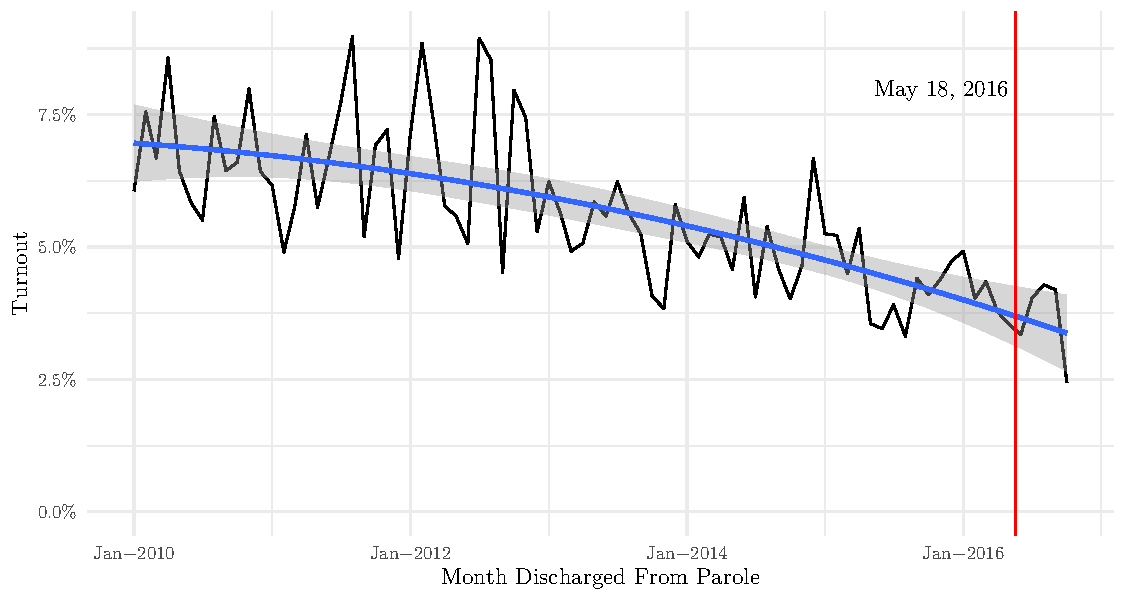
\includegraphics{part2_standalone_files/figure-latex/to-16-chart-1} 

}

\caption{\label{fig:to-16}Turnout in 2016 Presidential Election}\label{fig:to-16-chart}
\end{figure}

Figure \ref{fig:to-18} plots month of parole discharge and turnout in the 2018 midterm elections. Once again, a weighted quadratic curve is fitted with a 95 percent confidence band. This curve is fit on monthly data running from January 2012 through April 2018, and extended through October 2018.

\begin{figure}[H]

{\centering 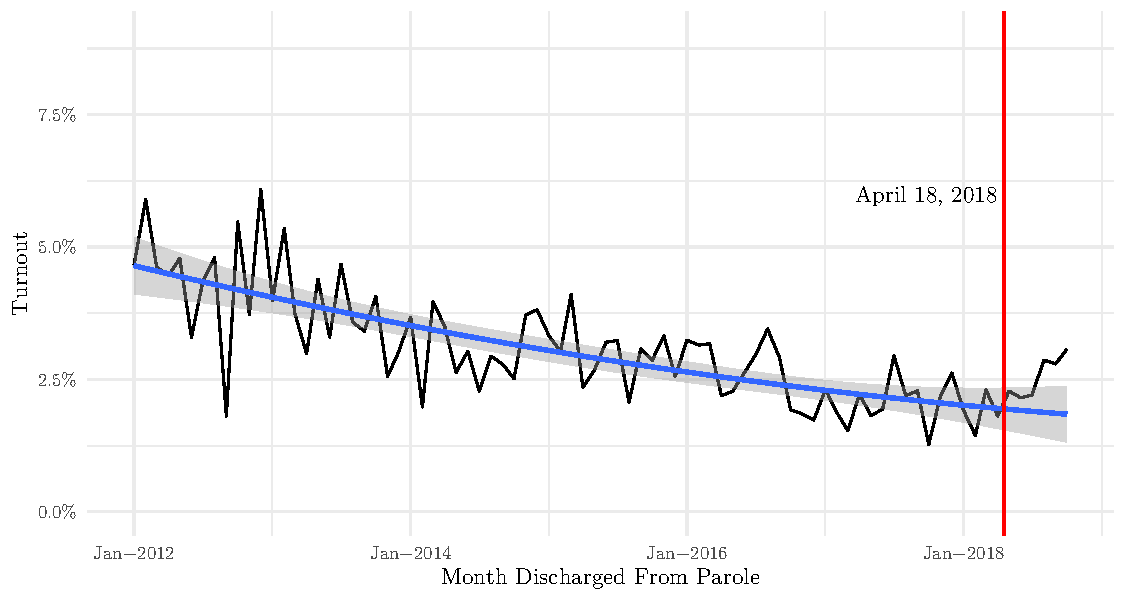
\includegraphics{part2_standalone_files/figure-latex/to-18-chart-1} 

}

\caption{\label{fig:to-18}Turnout in 2018 Midterm Election}\label{fig:to-18-chart}
\end{figure}

Figure \ref{fig:to-16} does not indicate that individuals who were discharged from parole shortly before the 2016 presidential election were more likely to cast a ballot than individuals discharged earlier in the year. Figure \ref{fig:to-18}, on the other hand, indicates that New Yorkers discharged from parole in the months leading up to the 2018 election --- many of whom had their rights restored while they were still on parole --- \emph{were} more likely to participate than those discharged earlier in the year. However, Figures \ref{fig:to-16} and \ref{fig:to-18} are noisy and do not prove that the executive order increased turnout.

\hypertarget{individual-level-turnout-regressions}{%
\subsection*{Individual-Level Turnout Regressions}\label{individual-level-turnout-regressions}}
\addcontentsline{toc}{subsection}{Individual-Level Turnout Regressions}

When considered over a multi-year period, the enactment of Executive Order 181 cannot be understood as a natural experiment. The longer an individual has been off of parole, the more likely she is to cast a ballot, but only individuals recently discharged from parole were eligible to have their voting rights restored prior to discharge. For a true natural experiment to hold, an individual's probability of being ``assigned'' to treatment (here, discharged from parole after the executive order went into effect) must be uncorrelated with the outcome of interest (propensity to vote). Figures \ref{fig:to-16} and \ref{fig:to-18} indicate that this is not the case when considering individuals discharged from parole over multiple years.

However, the relationship between time-off-parole and propensity to vote is far weaker in the short term. Figure \ref{fig:to-18-recent} indicates that parole discharge date and turnout rates in the 2018 midterm election are not correlated for individuals discharged in 2017 or 2018 before the executive order was enacted.

\begin{figure}[H]

{\centering 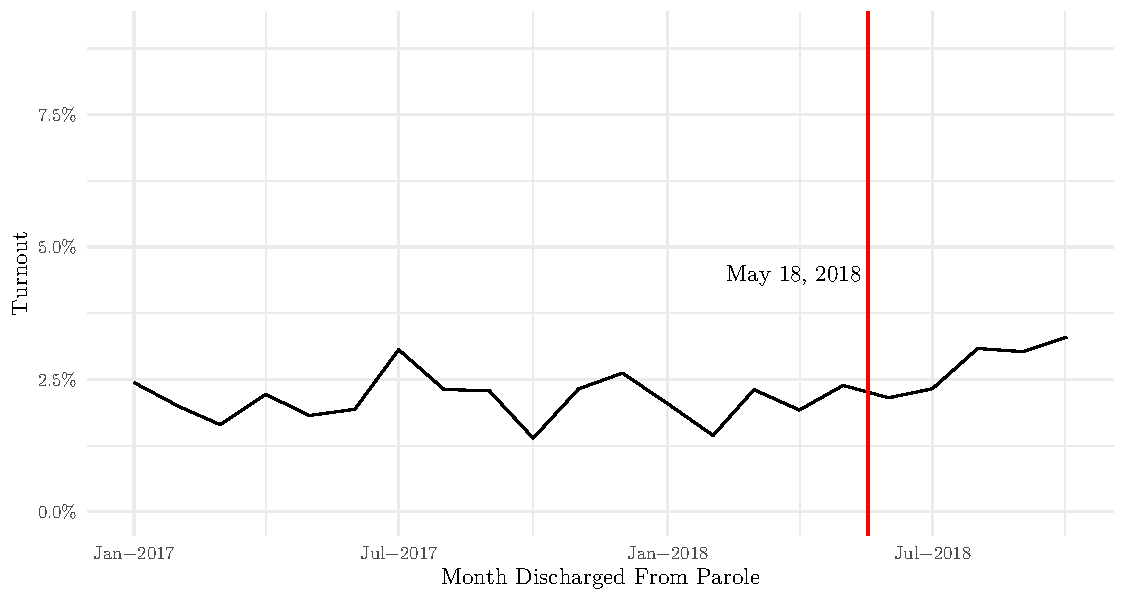
\includegraphics{part2_standalone_files/figure-latex/to-18-recent-chart-1} 

}

\caption{\label{fig:to-18-recent}Turnout in 2018 Midterm Election}\label{fig:to-18-recent-chart}
\end{figure}

Formalizing this chart into an individual-level logistic model demonstrates that time since discharge is not correlated with turnout in the short run. The models in Table \ref{tab:to-18-logit-short} include individuals last discharged from parole between January 1\textsuperscript{st}, 2017, and April 17\textsuperscript{th}, 2018 --- that is to say, all individuals discharged prior to the implementation of the executive order.

\input{"../../temp/table3.tex"}

The inclusion of time controls in Model 2 in Table \ref{tab:to-18-logit-short} leaves the AIC unchanged. A Chi-squared test confirms that the model is not improved when controls for time are included. When we look only at individuals recently discharged from parole, the length of time an individual has been off parole is not associated with his propensity to vote.\footnote{\protect\hyperlink{appendix-a}{Appendix A} provides further corroboration that being discharged from parole in the months before an election is uncorrelated with propensity to vote by exploring turnout rates in the 2016 presidential election.} This indicates that using individuals released in 2017 and 2018 prior to the executive order as a control group is feasible.

Although Governor Cuomo signed the executive order on April 18, 2018, an examination of the individuals whose rights were ultimately restored indicates that the program did not go into full effect until later in May. According to the rights restoration data, it is not until May 18\textsuperscript{th} that the majority of individuals discharged from parole had their rights restored prior to discharge.

Although it perhaps seems counterintuitive to throw out many of our observations, ignoring all individuals last discharged from parole prior to 2017 give us an important asset: it allows us to conceptualize Executive Order 181 as a natural experiment. Whether an individual was discharged from parole before or after May 18\textsuperscript{th}, 2018, is akin to a randomly assigned treatment. Individuals who were discharged from parole prior to the implementation of the executive order are part of the ``control group'', while individuals discharged after are assigned ``treatment'' by the policy change. Because Table \ref{tab:to-18-logit-short} shows that discharge date from parole is uncorrelated in the short term with an individual's propensity to vote, any observed difference in turnout between individuals discharged before and after late May can therefore be attributed to the executive order.

To further demonstrate the usefulness of discharge date as an intend-to-treat indicator, Table \ref{tab:demo-rd} shows the demographic characteristics of individuals in the control group (those discharged between January 1st, 2017, and May 17th, 2018) and the intend-to-treat group (those discharged between May 18th and October 12th, 2018). With the exception of age, the control and intend-to-treat groups are statistically indistinguishable from one another, further demonstrating the validity of the natural experiment conceptualization. The control group is, on average, slightly older, which Table \ref{tab:to-18-logit-short} indicates makes them slightly more likely to vote. To the extent our control group perhaps has a slightly higher propensity to vote than our intend-to-treat group our setup is (slightly) biased against finding a significant increase due to the executive order.

\input{"../../temp/table_whatever2.tex"}

In Table \ref{tab:to-18-logit}, I present the results of an individual-level logistic regression exploring whether individuals who were discharged on or after May 18\textsuperscript{th}, 2018, turned out at higher rates than those discharged earlier. The models include all individuals discharged from parole between January 1\textsuperscript{st}, 2017, through October 10\textsuperscript{th}, 2018 (the registration deadline in New York State).

\input{"../../temp/table4.tex"}

Model 1 in Table \ref{tab:to-18-logit} formalizes the trend presented in Figure \ref{fig:to-18-recent-chart} by controlling only for whether an individual was discharged after Executive Order 181 went into effect. Model 2 also controls for individual-level characteristics: sex, age on November 6\textsuperscript{th}, 2018, and race. Model 3 adds sentence-specific information to Model 2: the amount of time the individual spent on parole, and the class(es) of felony for which they were convicted. Table \ref{tab:to-18-logit} makes clear that formerly incarcerated men were far less likely to vote than formerly incarcerated women; that older formerly incarcerated individuals were more likely to cast a ballot; and individuals who spent longer on parole were more likely to participate in the midterm election.

Models 2 and 3 also indicate that individuals discharged from parole after the executive order went into effect were more likely to cast a ballot than those discharged earlier. Exponentiating the coefficients on D(Discharged After EO 181) indicates that Executive Order 181 raised the turnout rate among all formerly disenfranchised individuals by between 34.5 and 35 percent. The turnout rate for the control group was 2.1 percent.

\hypertarget{instrumental-variables-approach}{%
\subsection*{Instrumental Variables Approach}\label{instrumental-variables-approach}}
\addcontentsline{toc}{subsection}{Instrumental Variables Approach}

Table \ref{tab:to-18-logit} indicates that executive order was successful at increasing turnout among all formerly disenfranchised individuals. Although this intend-to-treat estimate is important information for policymakers and advocates hoping to increase the political representation of formerly incarcerated individuals as a whole, it does not shed light on the extent to which rights restoration increased the propensity to vote for the individuals who actually received the treatment. To answer that question, we must specifically control for whether an individual actually had his rights restored before he was discharged from parole --- not simply whether he was discharged after the policy change.

Investigating the causal effect of rights restoration using the natural experiment conceptualization introduces a complication: not all individuals who were discharged from parole after Executive Order 181 went into effect had their rights restored --- that is to say, not all individuals assigned to the treatment group ``complied.'' Noncitizens and individuals who violated their terms of parole were not eligible for rights restoration, and therefore did not ``comply'' with the treatment. Moreover, there is reason to suspect that compliance is correlated with propensity to vote.

An individual's propensity to vote can be expressed using the following equation:
\[ Y_i =  b_0 + b_{1}X_{1i} + b_{2}X_{2i} + b_{3}Z{i}+ \epsilon_{i} \]
Where \emph{Y\textsubscript{i}} is 1 if individual \emph{i} cast a ballot, \emph{X\textsubscript{1i}} is the probability that individual \emph{i} was eligible to have his rights restored prior to discharge from parole, and \emph{X\textsubscript{2i}} is 1 if individual \emph{i} actually had his rights restored prior to discharge from parole. \emph{Z} is a vector of other factors (such as age and race) known to influence voter turnout. Given that we cannot observe \emph{X\textsubscript{1i}}, we could simply choose to ignore it. Doing so, however, will result in consistent regression coefficients only if \emph{X\textsubscript{1i}} and \emph{X\textsubscript{2i}} (that is, eligibility to have rights restored, and actual restoration) are uncorrelated or if \emph{b\textsubscript{1}} is uncorrelated with an individual's propensity to vote (\emph{Y\textsubscript{i}}).

Neither of these assumptions are valid: firstly, an individual's eligibility to have her rights restored is certainly correlated with whether or not they actually were restored because the executive order required that all eligible individuals have their voting rights restored. Secondly, an individual's likelihood of having his rights restored is probably correlated with his natural propensity to vote. Individuals who were discharged from parole but are not U.S. citizens, for instance, did not having voting rights restored (or, in this case, granted) after the executive order went into effect. This ineligibility to have voting rights granted is of course correlated with these individuals' propensity to vote: non-citizens cannot cast ballots in elections in New York State. Table \ref{tab:demos-restorees} presents demographic differences between individuals who had their rights restored and those who did not among the intend-to-treat group (we cannot tell who would and would not have complied among the control group).

\input{"../../temp/table_whatever.tex"}

Table \ref{tab:demos-restorees} makes clear that the restoration of voting rights (``compliance'\,') is strongly correlated with certain demographics that are also linked to propensity to vote. Men, for instance, were less likely to have their rights restored than women, and Table \ref{tab:to-18-logit} above indicates that men who have been on probation are less likely to vote than women. Similarly, Latinos made up more than a third of individuals whose rights were not restored, but just 19 percent of individuals who did have voting rights restored. This is likely a reflection of citizenship status. Table \ref{tab:demos-restorees} indicates that \emph{b\textsubscript{1}} is very probably correlated with \emph{Y}. An approach in which is we regress turnout on a dummy indicating rights restoration is therefore inappropriate: such an approach cannot tell whether rights restoration \emph{caused} turnout to increase, or whether it simply identifies individuals with a higher propensity to vote.

The standard way of dealing with such a problem is an instrumental variables approach (Angrist, Imbens, and Rubin \protect\hyperlink{ref-Angrist1996}{1996}). Such an approach has been widely used in the context of voter turnout (e.g.~Ansolabehere, Iyengar, and Simon \protect\hyperlink{ref-Ansolabehere1999}{1999}; Gerber and Green \protect\hyperlink{ref-Gerber2000}{2000}; Milligan, Moretti, and Oreopoulos \protect\hyperlink{ref-Milligan2004}{2004}; Lassen \protect\hyperlink{ref-Lassen2004}{2004}; Sondheimer and Green \protect\hyperlink{ref-Sondheimer2010}{2010}). A valid instrumental variable must satisfy two criteria: it must be correlated with the right-hand-side (endogenous) variable of interest, and it must be uncorrelated with dependent variable (except via the endogenous variable).

In this case, such a variable is readily at hand. The likelihood that an individual had his voting rights restored is (in part) a function of whether he was discharged from parole after Executive Order 181 took effect. As demonstrated above, date of discharge from parole is not correlated with propensity to vote when we limit our analysis to individuals discharged from parole in 2017 or 2018. A dummy variable indicating whether an individual was discharged after the executive order was implemented, therefore, satisfies the criteria for an instrumental variable.

Two-stage least squares models allow us to leverage the random assignment of parole discharge date to identify the causal effect of rights restoration on the treated population --- what is often described as the ``local average treatment effect.'\,' The nature of our dependent variable (voting), instrumented variable (rights restoration), and instrument (discharge from parole before or after EO 181 went into effect) pose a challenge: each are binary values that can either be equal to 0 or 1. Linear models such as two-stage least squares do not ensure that the predicted probability of voting will fall on the {[}0, 1{]} interval. Although Angrist (\protect\hyperlink{ref-Angrist2001}{2001}) and Angrist and Pischke (\protect\hyperlink{ref-Angrist2008}{2008}) argue that in practice this limitation is usually trivial, the possibility remains that the linear model results in unacceptable misspecification. Some research (Gerber and Green \protect\hyperlink{ref-Gerber2000}{2000}; Green and Shachar \protect\hyperlink{ref-Green2000}{2000}; Lassen \protect\hyperlink{ref-Lassen2004}{2004}) using instrumental variables in the context of a binary vote-no vote framework has employed a two-stage probit (2S probit) model to avoid the constraints of the nonparametric framework. The 2S probit model specification, however, works best when the instrumented variable is continuous --- not, as in the case of rights restoration, a dichotomous variable (Dong and Lewbel \protect\hyperlink{ref-Dong2014}{2014}). The bivariate probit approach (see Wooldridge \protect\hyperlink{ref-Wooldridge2010}{2010}) is well suited for situations where the dependent variable, the instrumented variable, and instrument are all dichotomous (Terza, Bradford, and Dismuke \protect\hyperlink{ref-Terza2007}{2007}). This is especially true when the models exclude covariates and include only the dependent variable, the endogenous instrumented variable, and the instrument (Angrist \protect\hyperlink{ref-Angrist2001}{2001}).

Table \ref{tab:iv-models} presents the results of these various approaches on the question at hand. Models 1 and 2 utilize the linear two-stage least squares approach, with and without covariates. Model 3 uses the 2S probit specification (with all covariates), while Models 4 and 5 employ the bivariate probit specification (with and without covariates). For ease of comparison, I show the marginal effects of the probit models (measured at the means of the other variables).

\input{"../../temp/iv_clean.tex"}

The estimates of the bivariate probit model are modestly more conservative than the two-stage least squares model. After controlling for available demographics, the bivariate probit model indicates that rights restoration prior to discharge boosted turnout by individuals who had their rights restored by around 0.84 percentage points; the two-stage least squares model estimates that it increased turnout by around 0.96 percentage points. Though these numbers may seem small, they represent relatively large gains. Just 3.2 percent of individuals who had their rights restored cast a ballot in 2018, indicating that the executive order increased turnout by between 36.1 and 43.5 percent.

\hypertarget{racial-variation}{%
\subsubsection*{Racial Variation}\label{racial-variation}}
\addcontentsline{toc}{subsubsection}{Racial Variation}

Although these models demonstrate that rights restoration had a generally positive effect on participation in the 2018 election, the models hide substantial variation between races. In Table \ref{tab:iv-models-r} I present the two-stage least squares and bivariate probit models on subsets of former parolees. These models include only white former parolees (Models 1 and 4), all non-white former parolees (Models 2 and 5), and only black former parolees (Models 3 and 6). Once again, the marginal effects in the bivariate probit models are calculated at the means of the other variables.

\input{"../../temp/iv_clean_race.tex"}

Table \ref{tab:iv-models-r} indicates that rights restoration prior to discharge boosted turnout among white individuals by around 1.8 percentage points. Given that just 3.5 percent of white former parolees with restored voting rights cast a ballot, this means that rights restoration \emph{doubled} these individuals' likelihood of casting a ballot. We cannot determine whether rights restoration had an effect on non-white individuals: the coefficient on these estimates are small and not statistically significant.

Why would the intervention have increased turnout among white individuals and have had no effect on black individuals? Some of this may be explained by different propensities to vote. White (\protect\hyperlink{ref-White2019}{2019}), for instance, shows that brief periods of incarceration decreases black individuals' propensity to vote by substantially more than white individuals. She demonstrates that, prior to incarceration, black individuals were more likely to vote, identifying ``a narrative in which targeted policing brings many black defendants into court, including some voters (so they can be deterred), while lower arrest rates among whites mean that the white defendant pool rarely includes voters (so there is little demobilization, because the people jailed were unlikely to vote anyway)'' (321). The inverse may hold true here: if black individuals released from parole have a higher natural propensity to vote (even after accounting for potentially larger depressive effects from incarceration), they may be less susceptible to a policy intervention of this sort.

There is reason to believe this may be the case. Table \ref{tab:black-to} presents a series of logistic models estimating turnout in 2018 for the control group (individuals discharged from parole before the executive order went into effect), the intend-to-treat group (those discharged after the executive order), and of the treatment group (individuals whose rights were restored), testing whether black individuals turned out at higher rates. Because Latino voters are more likely to be non-citizens (and therefore have a lower turnout rate than black individuals), these individuals have been excluded from Models 2, 4, and 6 in case their inclusion overstates the relative propensity of black individuals to vote.

\input{"../../temp/table5.tex"}

Of the 14,155 individuals discharged from parole between January 1\textsuperscript{st}, 2017, and May 18\textsuperscript{th}, 2018, just over 6 thousand (43 percent) were black. These black voters were more than 50 percent more likely to vote in the midterms than the rest of the population. Even when Latinos are excluded from this group, black individuals were still a third more likely to cast a ballot. In both specifications, this higher turnout rate is significant at the 95 percent level of confidence.

Table \ref{tab:black-to} also shows, however, that among the intend-to-treat group (those discharged from parole after the executive order went into effect), black individuals were no more likely to participate in the 2018 general election. The same is true for the treatment group --- black individuals who had their rights restored were no more likely than other individuals to vote in 2018. The intervention, therefore, appears to have a leveling effect. Rights restoration prior to discharge seems to have no effect on future propensity to vote for black individuals, but that does not mean they are less likely to vote than other former parolees.

\hypertarget{variable-treatment-intensity}{%
\subsubsection*{Variable Treatment Intensity}\label{variable-treatment-intensity}}
\addcontentsline{toc}{subsubsection}{Variable Treatment Intensity}

There is some reason to believe that assuming a constant treatment effect understates the true impact of Executive Order 181. Figures \ref{fig:to-18-chart} and \ref{fig:to-18-recent-chart} suggest that, among individuals who finished parole after the Executive Order went into effect, individuals who were discharged later had a higher propensity to vote. This may be due to a number of factors: for instance, parole officers may have had longer to understand and communicate the new rules. Similarly, individuals discharged later may have had more meetings with their parole officers after the policy change, giving the parole officers multiple times to encourage the individuals under study to cast a ballot. Table \ref{tab:iv-models-time} investigates turnout as a function of the number of months an individual spent on parole after having her rights restored. If the individual did not have voting rights restored, this variable takes the value 0. This variable is instrumented by the number of months an individual spent on parole after the executive order went into effect. It is coded as 0 for individuals discharged prior to the implementation of the executive order.\footnote{Because the bivariate probit specification is not appropriate when the endogenous variable is not binary, that specification is not included in Table \ref{tab:iv-models-time}.}

\input{"../../temp/iv_clean_months.tex"}

Table \ref{tab:iv-models-time} indicates that variable treatment intensity matters --- individuals who spent longer on parole after they had their rights restored were more likely to vote than those whose rights were restored shortly before discharge. Table \ref{tab:iv-models-time} shows that for each month individuals spent on parole after having their rights restored, turnout increased by between 0.29 percentage points (in the 2SLS model) and 0.50 percentage points (in the 2S probit model).

Of course, with just a handful of months between the implementation of the executive order and the registration deadline for the 2018 midterms, it is impossible to know the full impact more months on parole after having one's rights restored has. One thing, however, is clear: focusing only on the individuals discharged from parole shortly after Executive Order 181 went into effect very likely underestimates the true impact it will have on parolee's propensity to vote when parolees spend more time under supervision with their rights formally restored.

\hypertarget{discussion}{%
\subsection*{Discussion}\label{discussion}}
\addcontentsline{toc}{subsection}{Discussion}

Restoring voting rights to individuals on parole is an important step toward undermining the disenfranchisement (both \emph{de jure} and \emph{de facto}) of communities of color disproportionately caught up in the criminal justice system. Prior to New York's Executive Order 181, parolees were required to wait until they finished their parole term to register to vote. That changed in 2018. On October 12\textsuperscript{th} --- the registration deadline for the 2018 midterms --- there were 21,863 active parolees whose voting rights had been restored. Without the executive order, every single one of these individuals would have been barred from participating. Though turnout among this group was low (just 832, or 3.81 percent, of these individuals successfully cast a ballot), their re-enfranchisement marks an important milestone for New York State.

As this analysis demonstrates, however, the impact of Executive Order 181 was not limited only to the individuals who would have been disenfranchised in its absence. In the case of New York State, rights restoration prior to discharge from parole is broadly successful at boosting post-supervision participation rates. In this project I estimate that rights restoration increased individuals' propensity to vote by at least 36.1 percent. This estimate, however, should be taken as a lower bound: the data indicate that individuals who spent longer on parole after having their rights restored were more likely to vote than individuals who were discharged immediately following the implementation of the Executive Order. Notably, this upward trend showed no signs of leveling off prior to the 2018 election; individuals whose rights were restored that were discharged in the fifth month after implementation voted at higher rates than those discharged after three months; those discharged after three months turned out at higher rates than those discharged in the first month.

The mechanism through which the rules change increased turnout among these individuals is not clear. Weaver and Lerman (\protect\hyperlink{ref-Weaver2010}{2010}) argues that contact with the criminal justice system restructures how individuals understand their relationship with the government and sours their desire to participate. Automatic voting rights restoration upon the completion of a sentence likely does little to combat these negative perceptions of the government. On the other hand, a parolee whose parole officer actively encourages them to register and participate may believe that the state is interested in their political participation. Such interactions may undo some of the negative socialization identified by Weaver and Lerman (\protect\hyperlink{ref-Weaver2010}{2010}).

It could also be a story of better information. As Meredith and Morse (\protect\hyperlink{ref-Meredith2015}{2015}) and Gerber et al. (\protect\hyperlink{ref-Gerber2014}{2014}) show, reminding formerly disenfranchised individuals of their restored voting rights can increase their participation (but see Meredith and Morse (\protect\hyperlink{ref-Meredith2013}{2013})). Research such as Manza and Uggen (\protect\hyperlink{ref-locked_out}{2006}) further demonstrates that many formerly incarcerated individuals wrongly believe that they are ineligible to participate. When a parolee has her voting rights restored prior to discharge --- and when her parole officer is required to inform her of that fact --- she is far more likely to be confident in her voting eligibility. The executive order likely meant that more formerly disenfranchised individuals were sure that they could cast a ballot in the 2018 election. In reality, the executive order's success at boosting turnout likely operated through multiple mechanisms.

Puzzlingly, the causal effect of pre-discharge rights restoration seems to vary based on parolees' race. Limiting the analysis to just White parolees reveals that rights restoration increased turnout by more than 90 percent. The fact that rights restoration prior to discharge appears to have no such impact on non-White or Black parolees is surprising given the magnitude of the effect for Whites. This discrepancy could be caused by a number of different factors. Firstly, Black and White individuals on parole might differ in meaningful ways that impact the successfulness of the intervention. As discussed above, Black participation among individuals discharged from parole prior to the executive order voted at significantly higher rates in 2018. The intervention was likely successful for parolees who would not have voted otherwise, but needed only a small encouragement. It may be that fewer Black former parolees are susceptible to small encouragements: they may separate more cleanly into voters and nonvoters, with fewer individuals susceptible to parole officer encouragement.

We cannot, however, rule out the possibility that racial bias among parole officers plays some role in the effectiveness of the intervention. Although parole officers may not be overtly or consciously biased toward their parolees, such bias is possible. Although there is limited literature examining racial variation in parolees' perceptions of their parole officers, there is some evidence that Black prisoners report worse inmate-staff relationships than White prisoners (Hemmens and Marquart \protect\hyperlink{ref-Hemmens2000}{2000}). Moreover, recent research indicates that street-level bureaucrats may exhibit some racial bias in the services they provide. White, Nathan, and Faller (\protect\hyperlink{ref-WHITE2014}{2014}), for instance, shows that local election administrators are less likely to respond to email questions from Latino aliases than non-Latino White aliases. There is also evidence that politicians are less likely to respond to requests from constituents of different races (Butler and Broockman \protect\hyperlink{ref-Butler2011}{2011}), and that public housing officials respond less to inquiries from Latinos (Einstein and Glick \protect\hyperlink{ref-Einstein2016}{2016}).

Parole officers may more enthusiastically encourage White parolees to register to vote and cast a ballot. This variation in encouragement would not necessarily be indicative of racial animus: it could arise from a parole officer's expectations about a parolee's political preferences. Officers are likely to provide greater encouragement to parolees they perceive to have similar political preferences. In the case of former parolees in New York State, race does serve as an effective proxy for partisanship: 82.5 percent of Black individuals discharged from parole since 2012 who participated in the 2018 election were registered Democrats; just 31.2 percent of such White individuals were registered Democrats. Ultimately, the data at hand cannot answer why the intervention succeeded at raising turnout only among White former parolees; future research must investigate why this is the case.

Re-enfranchising voters while they are still under formal supervision is obviously beneficial to the individuals who are on parole on election day; such policies allow them to make their voices heard. The case of Executive Order 181 also indicates that restoring voting rights prior to parole discharge has further benefits. In 2018, it increased turnout among individuals who were formally discharged from parole prior to the registration deadline, and therefore would have been eligible to vote even if their rights were not restored until the completion of their sentence. This is encouraging, demonstrating that the state has a unique opportunity to shape the future participation of individuals who are currently under their supervision. By restoring voting rights before individuals have completed their sentence, and by requiring parole officers to inform their parolees of their voting rights, the state can increase the political participation of a group of often-marginalized individuals, thereby increasing the democratic representation of our elections.

\newpage
\setcounter{table}{0}  \renewcommand{\thetable}{A\arabic{table}} \setcounter{figure}{0} \renewcommand{\thefigure}{A\arabic{figure}}

\hypertarget{appendix-a}{%
\section*{Appendix A}\label{appendix-a}}
\addcontentsline{toc}{section}{Appendix A}

In the \protect\hyperlink{instrumental-variables-approach}{Instrumental Variables Approach} section of this paper, I argue that being discharged from parole in the final months leading up to an election is uncorrelated with propensity to vote. Table \ref{tab:to-16-logit} demonstrates that individuals discharged between May 18\textsuperscript{th} -- October 14\textsuperscript{th}, 2016, did not participate at different rates in the 2016 presidential election than other formerly incarcerated individuals. Table \ref{tab:to-16-logit} includes all individuals last discharged from parole between January 1\textsuperscript{st}, 2015, and October 14\textsuperscript{th}, 2016.

\input{"../../temp/table55.tex"}

Although turnout was generally higher in 2016 than in 2018 (reflecting statewide higher turnout thanks to the presidential contest), there is no evidence that being discharged in the summer of 2016 was associated with an individual's propensity to cast a ballot. The nonsignificant results from 2016 provide strong corroboration that discharge date serves as an effective instrument for rights restoration.

\newpage

\hypertarget{references}{%
\section*{References}\label{references}}
\addcontentsline{toc}{section}{References}

\hypertarget{refs}{}
\begin{cslreferences}
\leavevmode\hypertarget{ref-Angrist2001}{}%
Angrist, Joshua D. 2001. ``Estimation of Limited Dependent Variable Models with Dummy Endogenous Regressors.'' \emph{Journal of Business \& Economic Statistics} 19 (1): 2--28. \url{https://doi.org/10.1198/07350010152472571}.

\leavevmode\hypertarget{ref-Angrist1996}{}%
Angrist, Joshua D., Guido W. Imbens, and Donald B. Rubin. 1996. ``Identification of Causal Effects Using Instrumental Variables.'' \emph{Journal of the American Statistical Association} 91 (434): 444--55. \url{https://doi.org/10.1080/01621459.1996.10476902}.

\leavevmode\hypertarget{ref-Angrist2008}{}%
Angrist, Joshua D., and Jörn-Steffen Pischke. 2008. \emph{Mostly Harmless Econometrics}. Princeton University Press. \url{https://doi.org/10.2307/j.ctvcm4j72}.

\leavevmode\hypertarget{ref-Ansolabehere1999}{}%
Ansolabehere, Stephen D., Shanto Iyengar, and Adam Simon. 1999. ``Replicating Experiments Using Aggregate and Survey Data: The Case of Negative Advertising and Turnout.'' \emph{American Political Science Review} 93 (4): 901--9. \url{https://doi.org/10.2307/2586120}.

\leavevmode\hypertarget{ref-bcj_laws}{}%
Brennan Center for Justice. 2018. ``Criminal Disenfranchisement Laws Across the United States.'' \url{https://www.brennancenter.org/criminal-disenfranchisement-laws-across-united-states}.

\leavevmode\hypertarget{ref-Burch2010}{}%
Burch, Traci. 2010. ``Did Disfranchisement Laws Help Elect President Bush? New Evidence on the Turnout Rates and Candidate Preferences of Florida's Ex-Felons.'' \emph{Political Behavior} 34 (1): 1--26. \url{https://doi.org/10.1007/s11109-010-9150-9}.

\leavevmode\hypertarget{ref-Burch2011}{}%
---------. 2011. ``Turnout and Party Registration Among Criminal Offenders in the 2008 General Election.'' \emph{Law and Society Review} 45 (3): 699--730. \url{https://doi.org/10.1111/j.1540-5893.2011.00448.x}.

\leavevmode\hypertarget{ref-Butler2011}{}%
Butler, Daniel M., and David E. Broockman. 2011. ``Do Politicians Racially Discriminate Against Constituents? A Field Experiment on State Legislators.'' \emph{American Journal of Political Science} 55 (3): 463--77. \url{https://doi.org/10.1111/j.1540-5907.2011.00515.x}.

\leavevmode\hypertarget{ref-Dong2014}{}%
Dong, Yingying, and Arthur Lewbel. 2014. ``A Simple Estimator for Binary Choice Models with Endogenous Regressors.'' \emph{Econometric Reviews} 34 (1-2): 82--105. \url{https://doi.org/10.1080/07474938.2014.944470}.

\leavevmode\hypertarget{ref-Drucker2005}{}%
Drucker, Ernest, and Ricardo Barreras. 2005. ``Studies of Voting Behavior and Felony Disenfranchisement Among Individuals in the Criminal Justice System in New York, Connecticut, and Ohio.'' Research report. Sentencing Project. \url{https://www.prisonpolicy.org/scans/sp/fd_studiesvotingbehavior.pdf}.

\leavevmode\hypertarget{ref-Einstein2016}{}%
Einstein, Katherine Levine, and David M. Glick. 2016. ``Does Race Affect Access to Government Services? An Experiment Exploring Street-Level Bureaucrats and Access to Public Housing.'' \emph{American Journal of Political Science} 61 (1): 100--116. \url{https://doi.org/10.1111/ajps.12252}.

\leavevmode\hypertarget{ref-Gerber2000}{}%
Gerber, Alan S., and Donald P. Green. 2000. ``The Effects of Canvassing, Telephone Calls, and Direct Mail on Voter Turnout: A Field Experiment.'' \emph{American Political Science Review} 94 (3): 653--63. \url{https://doi.org/10.2307/2585837}.

\leavevmode\hypertarget{ref-Gerber2014}{}%
Gerber, Alan S., Gregory A. Huber, Marc Meredith, Daniel R. Biggers, and David J. Hendry. 2014. ``Can Incarcerated Felons Be (Re)integrated into the Political System? Results from a Field Experiment.'' \emph{American Journal of Political Science} 59 (4): 912--26. \url{https://doi.org/10.1111/ajps.12166}.

\leavevmode\hypertarget{ref-Gerber2017}{}%
---------. 2017. ``Does Incarceration Reduce Voting? Evidence About the Political Consequences of Spending Time in Prison.'' \emph{The Journal of Politics} 79 (4): 1130--46. \url{https://doi.org/10.1086/692670}.

\leavevmode\hypertarget{ref-Green2000}{}%
Green, Donald P., and Ron Shachar. 2000. ``Habit Formation and Political Behaviour: Evidence of Consuetude in Voter Turnout.'' \emph{British Journal of Political Science} 30 (4): 561--73. \url{https://doi.org/10.1017/s0007123400000247}.

\leavevmode\hypertarget{ref-Haselswerdt2009}{}%
Haselswerdt, Michael V. 2009. ``Con Job: An Estimate of Ex-Felon Voter Turnout Using Document-Based Data.'' \emph{Social Science Quarterly} 90 (2): 262--73. \url{https://doi.org/10.1111/j.1540-6237.2009.00616.x}.

\leavevmode\hypertarget{ref-Hemmens2000}{}%
Hemmens, Craig, and James W. Marquart. 2000. ``Friend or Foe? Race, Age, and Inmate Perceptions of Inmate-Staff Relations.'' \emph{Journal of Criminal Justice} 28 (4): 297--312. \url{https://doi.org/10.1016/s0047-2352(00)00044-1}.

\leavevmode\hypertarget{ref-Lassen2004}{}%
Lassen, David Dreyer. 2004. ``The Effect of Information on Voter Turnout: Evidence from a Natural Experiment.'' \emph{SSRN Electronic Journal}. \url{https://doi.org/10.2139/ssrn.475821}.

\leavevmode\hypertarget{ref-locked_out}{}%
Manza, Jeff, and Christopher Uggen. 2006. \emph{Locked Out: Felon Disenfranchisement and American Democracy}. New York: Oxford University Press.

\leavevmode\hypertarget{ref-Meredith2013}{}%
Meredith, Marc, and Michael Morse. 2013. ``Do Voting Rights Notification Laws Increase Ex-Felon Turnout?'' Edited by Christopher Wildeman, Jacob S. Hacker, and Vesla M. Weaver. \emph{The ANNALS of the American Academy of Political and Social Science} 651 (1): 220--49. \url{https://doi.org/10.1177/0002716213502931}.

\leavevmode\hypertarget{ref-Meredith2015}{}%
---------. 2015. ``The Politics of the Restoration of Ex-Felon Voting Rights: The Case of Iowa.'' \emph{Quarterly Journal of Political Science} 10 (1): 41--100. \url{https://doi.org/10.1561/100.00013026}.

\leavevmode\hypertarget{ref-Milligan2004}{}%
Milligan, Kevin, Enrico Moretti, and Philip Oreopoulos. 2004. ``Does Education Improve Citizenship? Evidence from the United States and the United Kingdom.'' \emph{Journal of Public Economics} 88 (9-10): 1667--95. \url{https://doi.org/10.1016/j.jpubeco.2003.10.005}.

\leavevmode\hypertarget{ref-Pierson1993}{}%
Pierson, Paul. 1993. ``When Effect Becomes Cause: Policy Feedback and Political Change.'' \emph{World Politics} 45 (4): 595--628. \url{https://doi.org/10.2307/2950710}.

\leavevmode\hypertarget{ref-Sondheimer2010}{}%
Sondheimer, Rachel Milstein, and Donald P. Green. 2010. ``Using Experiments to Estimate the Effects of Education on Voter Turnout.'' \emph{American Journal of Political Science} 54 (1): 174--89. \url{https://doi.org/10.1111/j.1540-5907.2009.00425.x}.

\leavevmode\hypertarget{ref-Terza2007}{}%
Terza, Joseph V., W. David Bradford, and Clara E. Dismuke. 2007. ``The Use of Linear Instrumental Variables Methods in Health Services Research and Health Economics: A Cautionary Note.'' \emph{Health Services Research} 43 (3): 1102--20. \url{https://doi.org/10.1111/j.1475-6773.2007.00807.x}.

\leavevmode\hypertarget{ref-sentencing_2016}{}%
Uggen, Christopher, Ryan Larson, and Sarah Shannon. 2016. ``6 Million Lost Voters: State-Level Estimates of Felony Disenfranchisement, 2016.'' Research report. Sentencing Project. \url{https://www.sentencingproject.org/publications/6-million-lost-voters-state-level-estimates-felony-disenfranchisement-2016/}.

\leavevmode\hypertarget{ref-Uggen2004}{}%
Uggen, Christopher, and Jeff Manza. 2004. ``Lost Voices: The Civic and Political Views of Disfranchised Felons.'' In \emph{Imprisoning America: The Social Effects of Mass Incarceration}, edited by Mary Pattillo, David Weiman, and Bruce Western, 165--204. New York: Russell Sage Foundation.

\leavevmode\hypertarget{ref-Uggen2002}{}%
---------. 2002. ``Democratic Contraction? Political Consequences of Felon Disenfranchisement in the United States.'' \emph{American Sociological Review} 67 (6): 777. \url{https://doi.org/10.2307/3088970}.

\leavevmode\hypertarget{ref-Weaver2010}{}%
Weaver, Vesla M., and Amy E. Lerman. 2010. ``Political Consequences of the Carceral State.'' \emph{American Political Science Review} 104 (4): 817--33. \url{https://doi.org/10.1017/s0003055410000456}.

\leavevmode\hypertarget{ref-White2019}{}%
White, Ariel. 2019. ``Misdemeanor Disenfranchisement? The Demobilizing Effects of Brief Jail Spells on Potential Voters.'' \emph{American Political Science Review} 113 (2): 311--24. \url{https://doi.org/10.1017/s000305541800093x}.

\leavevmode\hypertarget{ref-WHITE2014}{}%
White, Ariel, Noah Nathan, and Julie Faller. 2014. ``What Do I Need to Vote? Bureaucratic Discretion and Discrimination by Local Election Officials.'' \emph{American Political Science Review} 109 (1): 129--42. \url{https://doi.org/10.1017/s0003055414000562}.

\leavevmode\hypertarget{ref-Wooldridge2010}{}%
Wooldridge, Jeffrey M. 2010. \emph{Econometric Analysis of Cross Section and Panel Data}. Cambridge, MA: The MIT Press.
\end{cslreferences}

\end{document}
